%% LyX 2.3.6 created this file.  For more info, see http://www.lyx.org/.
%% Do not edit unless you really know what you are doing.
\documentclass[english]{scrartcl}
\usepackage[T1]{fontenc}
\usepackage[latin9]{inputenc}
\usepackage{graphicx}
\usepackage{babel}
\usepackage{listings}
\renewcommand{\lstlistingname}{Listing}

\begin{document}
\title{SEA3004F MEMO: Matrix manipulations\\
Ocean and Atmosphere Dynamics}
\maketitle

\section{Tutorial {[}20{]}}

Check if the student has included all the sections of the tutorial
as done in class. 
\begin{enumerate}
\item Markup cells with section titles: 5 points
\item Comments in code cells: 7
\item figures of the house and rotated house: 4 each
\end{enumerate}

\section{Exercise 1 {[}20{]}}

A perfect code like the one below is 20. 
\begin{itemize}
\item Vector: 5
\item Rotation matrix: 10 
\item Figures: 5 each
\end{itemize}
\begin{lstlisting}[language=Matlab,basicstyle={\footnotesize}]
>> V = [ -1  -1  -3   0   3   1   1; -5   5   5   8   5   5  -5  ];
>> figure(1)
>> dot2dot(V)
>> print -f1 -dpng -r100 fig1.png
>> theta=-pi+pi/6
theta =
   -1.0472
>> G = [cos(theta) -sin(theta); sin(theta) cos(theta)]
G =
   -0.8660    0.5000
   -0.5000   -0.8660
>> W=G*V
W =
   -1.6340    3.3660    5.0981    4.0000   -0.0981    1.6340   -3.3660
    4.8301   -3.8301   -2.8301   -6.9282   -5.8301   -4.8301    3.8301
>> figure(2)
>> dot2dot(W)
>> print -f2 -dpng -r100 fig2.png
\end{lstlisting}

\begin{figure}
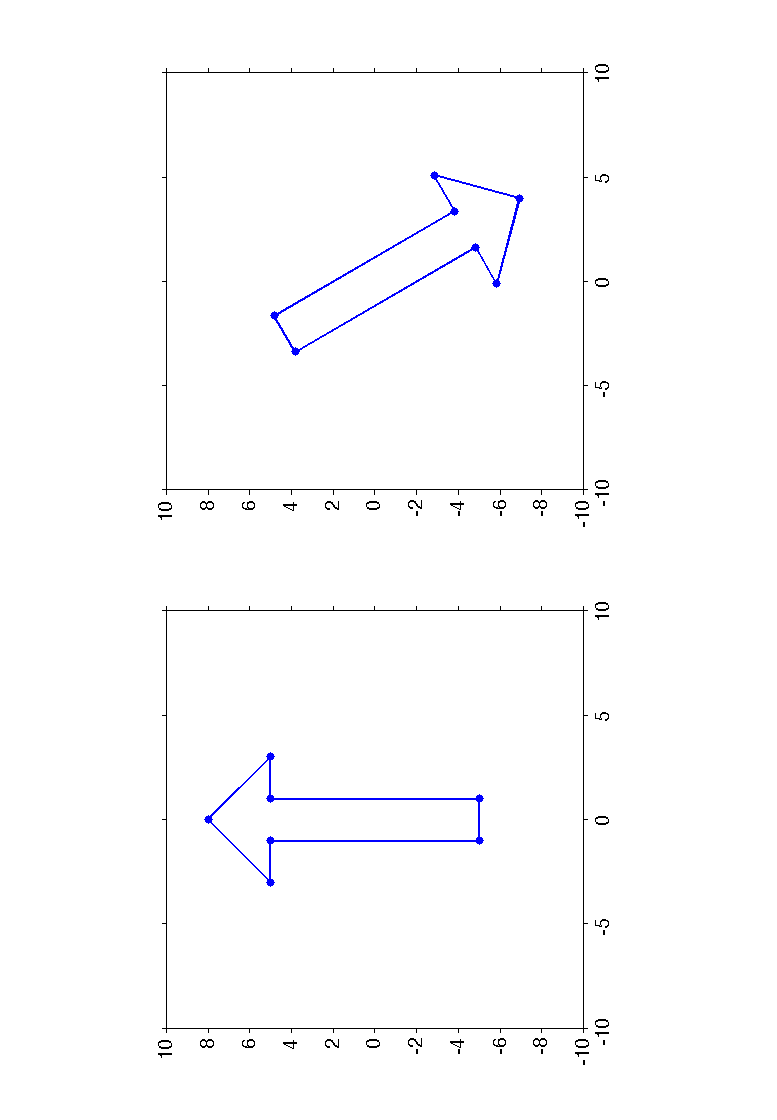
\includegraphics[angle=-90,scale=0.5]{fig1}

\caption{The original and rotated vectors}
\end{figure}

\end{document}
